\section{Background and Motivation}
\label{sec:background}

\subsection{Partitioned Inference on a Coherent Edge SoC}

Thor's MIG profiles divide GPU execution resources and isolate MIG-local
allocations.  We use one 1g instance with eight streaming multiprocessors and
one 2g instance with twelve.  Each stage owns a distinct CUDA context and an
opaque, serialized TensorRT engine.  This is a useful fault and resource
boundary, but it is not an inter-stage data plane: a device allocation made by
the producer cannot simply become the consumer's binding.

The integrated memory architecture creates a second, orthogonal property.
CPU mappings and the iGPU ultimately reach the same physical SoC DRAM.  CUDA
can register a page-aligned system-memory range in each process and return a
context-local device pointer for that range.  The producer and consumer
therefore use different virtual device pointers to the same physical payload.
MIG isolation remains intact because neither process imports the other's
MIG-local allocation.

This distinction determines our terminology.  The implemented transport is a
\emph{full-coherent registered system-memory activation edge}.  It is not
\texttt{cudaMallocManaged}/UVM.  It also does not imply free communication:
the request still incurs publication ordering, a CPU notification, consumer
wakeup, and contention on shared SoC resources.  \sys treats those costs as
measured properties of a placement rather than attributes of the memory API.

\subsection{Why Independent-Client Provisioning Falls Short}

Consider a producer $P$, a consumer $C$, and an unrelated best-effort tenant
$B$.  A fixed spatial policy can isolate $P$ and $C$, and an MPS quota can
limit $B$ within the producer instance.  Neither policy represents the
precedence $P\prec C$.  Three consequences follow.

\textbf{The edge is outside the resource model.}
The provisioner can select two partitions without knowing the payload size,
transport, or notification tail between them.  Treating these quantities as a
constant copy term is incorrect on a coherent SoC: cache state and overlapping
GPU or memory traffic can dominate the measured handoff.

\textbf{Protection has no release event.}
Pausing $B$ for the complete request protects both stages but wastes the
interval in which only $C$ runs on the other partition.  Keeping $B$ active
throughout the request permits already-issued work to delay $P$.  The
activation's publication is the earliest event that is both safe and useful
for returning the producer's capacity.

\textbf{Tail objectives are not end-to-end SLOs.}
Adding independently measured p99s is not a p99 bound: tail events need not
occur on the same request.  Admission must use either the measured joint
arrival-to-completion distribution or an explicit risk allocation, and it
must include gate acquisition and queue delay.

\begin{table}[t]
  \centering
  \small
  \caption{Scheduling scope under the dependent two-stage contract.  A cross
  means that the abstraction does not expose the property as a first-class
  contract; it does not preclude composing additional software around it.}
  \label{tab:abstraction-gap}
  \resizebox{\columnwidth}{!}{%
  \begin{tabular}{lcccc}
    \toprule
    Abstraction & Isolated placement & Explicit activation & Publication release & E2E admission \\
    \midrule
    MIG / MPS & \cmark & \xmark & \xmark & \xmark \\
    Independent-service provisioner & \cmark & \xmark & \xmark & partial \\
    Kernel / stream scheduler & partial & \xmark & \xmark & partial \\
    \textbf{\sys} & \cmark & \cmark & \cmark & \cmark \\
    \bottomrule
  \end{tabular}%
  }
\end{table}

Table~\ref{tab:abstraction-gap} summarizes the gap.  \sys does not replace
hardware isolation or fine-grained scheduling.  It adds the dependency,
publication, and deadline contracts required to use those mechanisms for a
cross-partition pipeline.

\subsection{A Request-Rate Crossover}

Isolation is sufficient when the dependent stages fit comfortably inside one
instance.  Our ImageNette control is in this regime: its consumer is much
shorter than its producer, and colocating both stages on 2g avoids an
unproductive split.  The relevant counterexample is a pipeline with substantial
work on both sides of the edge and more than one request in flight.

We test that counterexample with the real encoder and decoder of
Whisper-Tiny~\cite{radford2022whisper}.  Three activation slots allow encoder
request $i+1$ on 1g to overlap decoder request $i$ on 2g.  Every arm replays the
same labelled LibriSpeech windows, $2{,}304{,}000$-byte FP32 activation,
19-request/s release schedule, $250$-ms deadline, saturated DistilBERT
best-effort tenant, and output oracle.  We rotate the treatment order over
three sessions of 100 measured requests.  NVIDIA MIG places both critical
stages on 2g and isolates best effort on 1g; static NVIDIA MPS splits the
stages but continuously shares 1g; \sys uses the same split and protects 1g
only through producer publication.  TensorRT requires profile-specific
encoder plans, so we rebuild and hash-bind 1g and 2g FP32 plans while holding
the model, decoder plans, inputs, and outputs fixed.

\begin{figure*}[t]
  \centering
  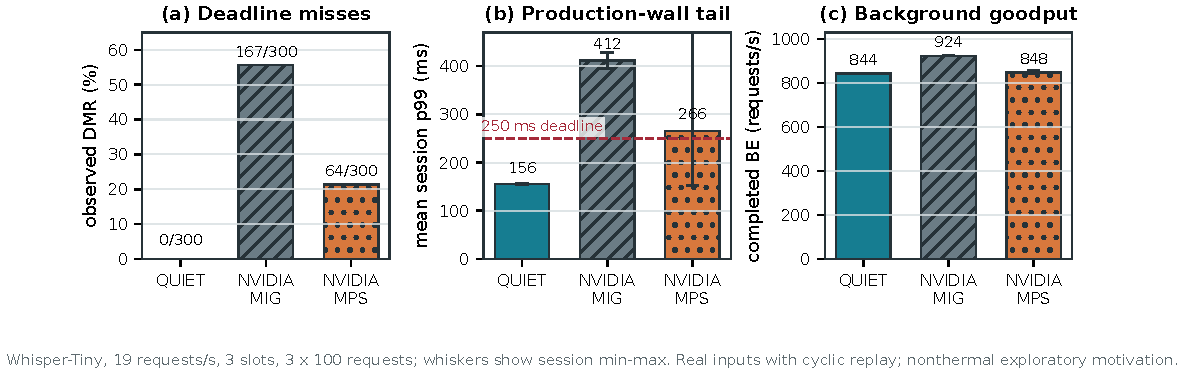
\includegraphics[width=\textwidth]{figures/p9-whisper-asr-mig-crossover.pdf}
  \caption{Nonthermal Whisper-ASR motivation at 19 requests/s.  Every panel
  repeats \sys, NVIDIA MIG, and NVIDIA MPS in the same order.  Bars aggregate
  three 100-request sessions; p99 and best-effort whiskers show the session
  range.  The twelve real windows are cyclically replayed for performance and
  do not constitute additional accuracy coverage.}
  \label{fig:asr-mig-crossover}
  \Description{Three bar charts compare QUIET, NVIDIA MIG, and NVIDIA MPS.
  QUIET has zero of 300 deadline misses and 156 ms mean session p99.  MIG has
  167 misses and 412 ms p99.  MPS has 64 misses and 266 ms p99.  MIG has the
  highest background goodput; QUIET and MPS have similar background goodput.}
\end{figure*}

Figure~\ref{fig:asr-mig-crossover} exposes the crossover.  MIG misses 167 of
300 deadlines because co-located stages sustain only 17.791 requests/s and
queue p99 reaches 241.104 ms.  Static MPS misses 64 requests, all in one
session.  \sys records 0/300 misses, a 155.581-ms mean session p99, and 18.732
critical requests/s.  Its 843.645 best-effort requests/s differs by only
$-0.5\%$ from static MPS, while MIG preserves 924.073 requests/s by dedicating
1g to best effort.  All nine output traces are byte-identical.  The result
therefore identifies a dependency-rate regime in which rigid isolation is not
the correct placement and ungated sharing is not stable enough.

The architecture and dependency are deployment-real, but the load point is
only partially so.  Thor officially supports concurrent hardware-isolated tenants in this 1g+2g
geometry~\cite{nvidiathormig}; Whisper is a real 30-second-window
encoder--decoder application, and prior work adapts it to live streaming
service~\cite{machacek2023whisperstreaming}.  Our fixed 19-request/s trace can
represent a multi-channel edge gateway or queued transcription service, but it
is a cyclic replay rather than a measured deployment arrival trace.  The
250-ms deadline is an internal inference budget, not a universal ASR response
target.  We consequently use Figure~\ref{fig:asr-mig-crossover} as nonthermal
motivation, not as a formal headline or accuracy expansion.

\subsection{Execution and Evidence Contract}

For request $i$, let $a_i$ be its actual release and $c_i$ the consumer's
production completion.  The measured response is
\begin{equation}
  L_i = c_i-a_i ,
  \label{eq:production-wall}
\end{equation}
and a deadline miss occurs when $L_i>D$.  A declared release is never moved
forward to hide a busy pipeline.  If the runtime reaches it late, the
difference is recorded as queue delay and remains inside $L_i$.  Checksum and
output-oracle work occurs after $c_i$; its duration is recorded but cannot
inflate the service metric or extend the protection interval.

The current promoted runtime executes a two-stage chain with at most one
request in flight in each process.  A separate three-slot, external-process
ring validates ownership, wraparound, backpressure, bounded timeout, and stale
slot reclamation, but it is not yet the production TensorRT path.  Likewise,
the planner schema validates larger DAG topologies, while the executed
application remains two-stage.  We therefore make neither a general-DAG nor a
multi-inflight performance claim.

These constraints lead to four design requirements:
\begin{enumerate}[leftmargin=*,itemsep=1pt,topsep=2pt]
  \item \textbf{R1: exact payload semantics.}  Both stages must bind the full
  request-specific activation, with no token or constant-payload substitute.
  \item \textbf{R2: publication-scoped protection.}  The best-effort tenant
  must be acknowledged idle before producer release and resumed immediately
  after payload visibility.
  \item \textbf{R3: joint-tail admission.}  Placement and quotas must fit a
  frozen arrival-to-completion deadline using a promotable tail model.
  \item \textbf{R4: fail-closed evidence.}  A stale engine, binary, input,
  release trace, plan, or output must invalidate the result rather than
  silently changing its contract.
\end{enumerate}
